\chapter{Introduction to molecular dynamics simulations with NAMD and VMD}

Thermal neutron scattering, which is sensitive to the dynamics and the structure of condensed matter on the atomic scale, gives precise information about atomic fluctuations and dynamics in proteins, enhancing an average view of all atomic contributions.
In this way, as seen in section \ref{}, with simple analytical models it is possible to analyze some basic feautures of the protein spectra. However, due to the high complexity of these system, usually their internal dynamics is too complicated to for a quantitative interpretation in terms of such models based almost only upon average information. 

To overcome this limitation of neutron scattering it is possible to use computer simulations, and in particular Molecular Dynamics (MD) simulations, that enable to gain a wider insight into the dynamics of proteins that are not provided from the neutron scattering experiments. The combination of both methods access in the same time and space domains, and the comparison of simulated and measured spectra is thouroughly direct, since neutrons are diffused by the atomic nuclei (neglecting magnetic scattering), which are the actual objects of study of MD simulations. Once an alignment between simulated and experimental spectra is found, thus the experimental data supports the data obtained from the computer simulation, then the simulated trajectories can be analyzed in detail and information not accessible from experiments can be extracted from computer simulations.

In this sense, computer simulations that are built upon the actual experimental data, can overcome the limitations of neutron scattering and grasp the more complex spectra of the proteins.\footnote{Some iteresting applications, relevant to the interpretation of quasielastic neutron scattering and concerning the simulation-based development of models for slow protein dynamics, are discussed in Kneller's lecture \cite{ref:QNS_Keller}.}

\section{Introduction to molecular dynamics simulations}
MD simulations are one of the principal tools in the theoretical study of biomolecules providing informations on thermal fluctations of atoms in a molecule as well as informations about relative positions of molecules and atoms in dependence of time. In fact, MD is a computational method which allows to calculate the time dependent behavior of complex molecular system (e.g. proteins, enzymes, etc.) and hence it is generally used to describe such systems in terms of a realistic atomic model, with an aim to understand and predict macroscopic properties based on detailed knowledge on an atomic scale. Indeed, starting from an atomistic level, MD simulations are used to predict and better understand the properties of complex materials. In this way MD provide a direct route from the microscopic details of a system (the masses of the atoms, the interactions between them, etc.) to macroscopic properties of experimental interest (the equation of state, transport coefficients and so on). In particular, usually biomolecular MD simulations are used to gain insight into ligand binding, enzymatic activities, signalling mechanisms and protein folding \cite{ref:NAMD-VMD_Kukol}. Additionally simulations are valuable tools for the refinement of electron microscopy, x-ray, inelastic neutron scattering or other spectroscopic data in order to obtain more accurate molecular structures.

More to the point, MD simulations compute the motions of individual molecules for a classical many-body system in order to describe the equilibrium and transport properties of solids, liquids and gasses.
Although this modelling of the matter at the microscopic level must be, in principle, based on quantum mechanics, MD generally adopts a classical point of view.
In this context, the word classical means that the nuclear motion of the constituent particles obeys the laws of classical mechanics (the motion is described by the second Newton's law).
This is an excellent approximation for a wide range of materials.

Hence, in MD neither relativistic nor quantum effects are considered:
\begin{itemize}
\item[$\circ$] \textit{Special relativity} does not allow information to travel faster than light; MD simulations assume forces with an infinite speed of propagation.
\item[$\circ$] \textit{Quantum mechanics} has at its base the uncertainty principle; MD requires, and provides, complete information about position and momentum at all times.
\end{itemize}

In practice, the phenomena studied by MD simulations are those where relativistic effects are not observed and quantum effects can, if necessary, be incorporated as semi-classical corrections derived from quantum theory.\footnote{For example, dealing with very light atoms or molecules (e.g. He, H$_2$, D$_2$) or with vibrational motions with characteristic energy comparable or larger than $k_B T$, quantum effects became not negligible.}
% whose characteristic frequency, translated in energy, is comparable or larger than $k_B T$, quantum effects became not negligible.}

MD simulations allow to calculate several properties of many-particle systems. However, not all properties can be directly measured in a simulation. Conversely, most of the quantities that can be measured in a simulation do not correspond to properties that are measured in real experiments.
Actually, molecular simulations generate information at the microscopic level (atomic and molecular positions, velocities, etc.) and the conversion of this very detailed information into macroscopic terms (pressure, internal energy, etc.) is the field of the statistical mechanics. Thus, the language of statistical mechanics is necessary to use these simulations as the numerical counterpart of experiments.

In this context, it is useful to see that there is a direct connection between MD simulations and the microcanonical ensemble of statistical mechanics. Indeed, the microcanonical ensemble consists of all microscopic states $( \bold{r}^N(t), \, \bold{p}^N(t) )$  on the constant energy hypersurface $H (\bold{r}^N(t) , \, \bold{p}^N(t)) \:=\: E$.
On the other hand, the classical Hamiltonian mechanics the equations of motion conserve the total energy: 
\begin{equation}\label{eq:hamilton-energy_cons}
\frac{dH}{dt} \:=\: 0 \quad \Longrightarrow \quad H ( \bold{r}^N(t), \, \bold{p}^N(t) ) \:=\: const.
\end{equation}

This suggests a link between the microcanonical ensemble and classical Hamiltonian mechanics. In fact, for a system that evolves according to Hamilton's equations of motion:
\begin{equation}\label{eq:hamilton}
\dot{\bold{r}}_i(t) \:=\: \frac{\partial H}{\partial \bold{p}_i} \qquad \qquad \dot{\bold{p}}_i(t) \:=\: - \frac{\partial H}{\partial \bold{r}_i}
\end{equation}
a trajectory computed with these equations will generate microscopic configurations belonging to the microcanonical ensemble with the constant energy $E$. Thus, if after a long time a system with energy $E$ is able to visit practically all the configurations on the constant energy hypersurface, the dynamical evolution of this system can be used to generate a micro-canonical ensemble. A system that has this property is said to be \textit{ergodic}.

In general this dynamical approach, that is at the basis of MD simulations, provides a powerful method for generating an ensemble and its averages.\footnote{In MD programs the phase of the simulation used to generate the ensemble is usually named: \textit{equilibration}.} Thus MD simulations have evolved into one of the most widely used techniques for solving statistical mechanical problems.

\begin{figure}[H]
\centering
\begin{minipage}[t]{0.75\textwidth}
	\centering
    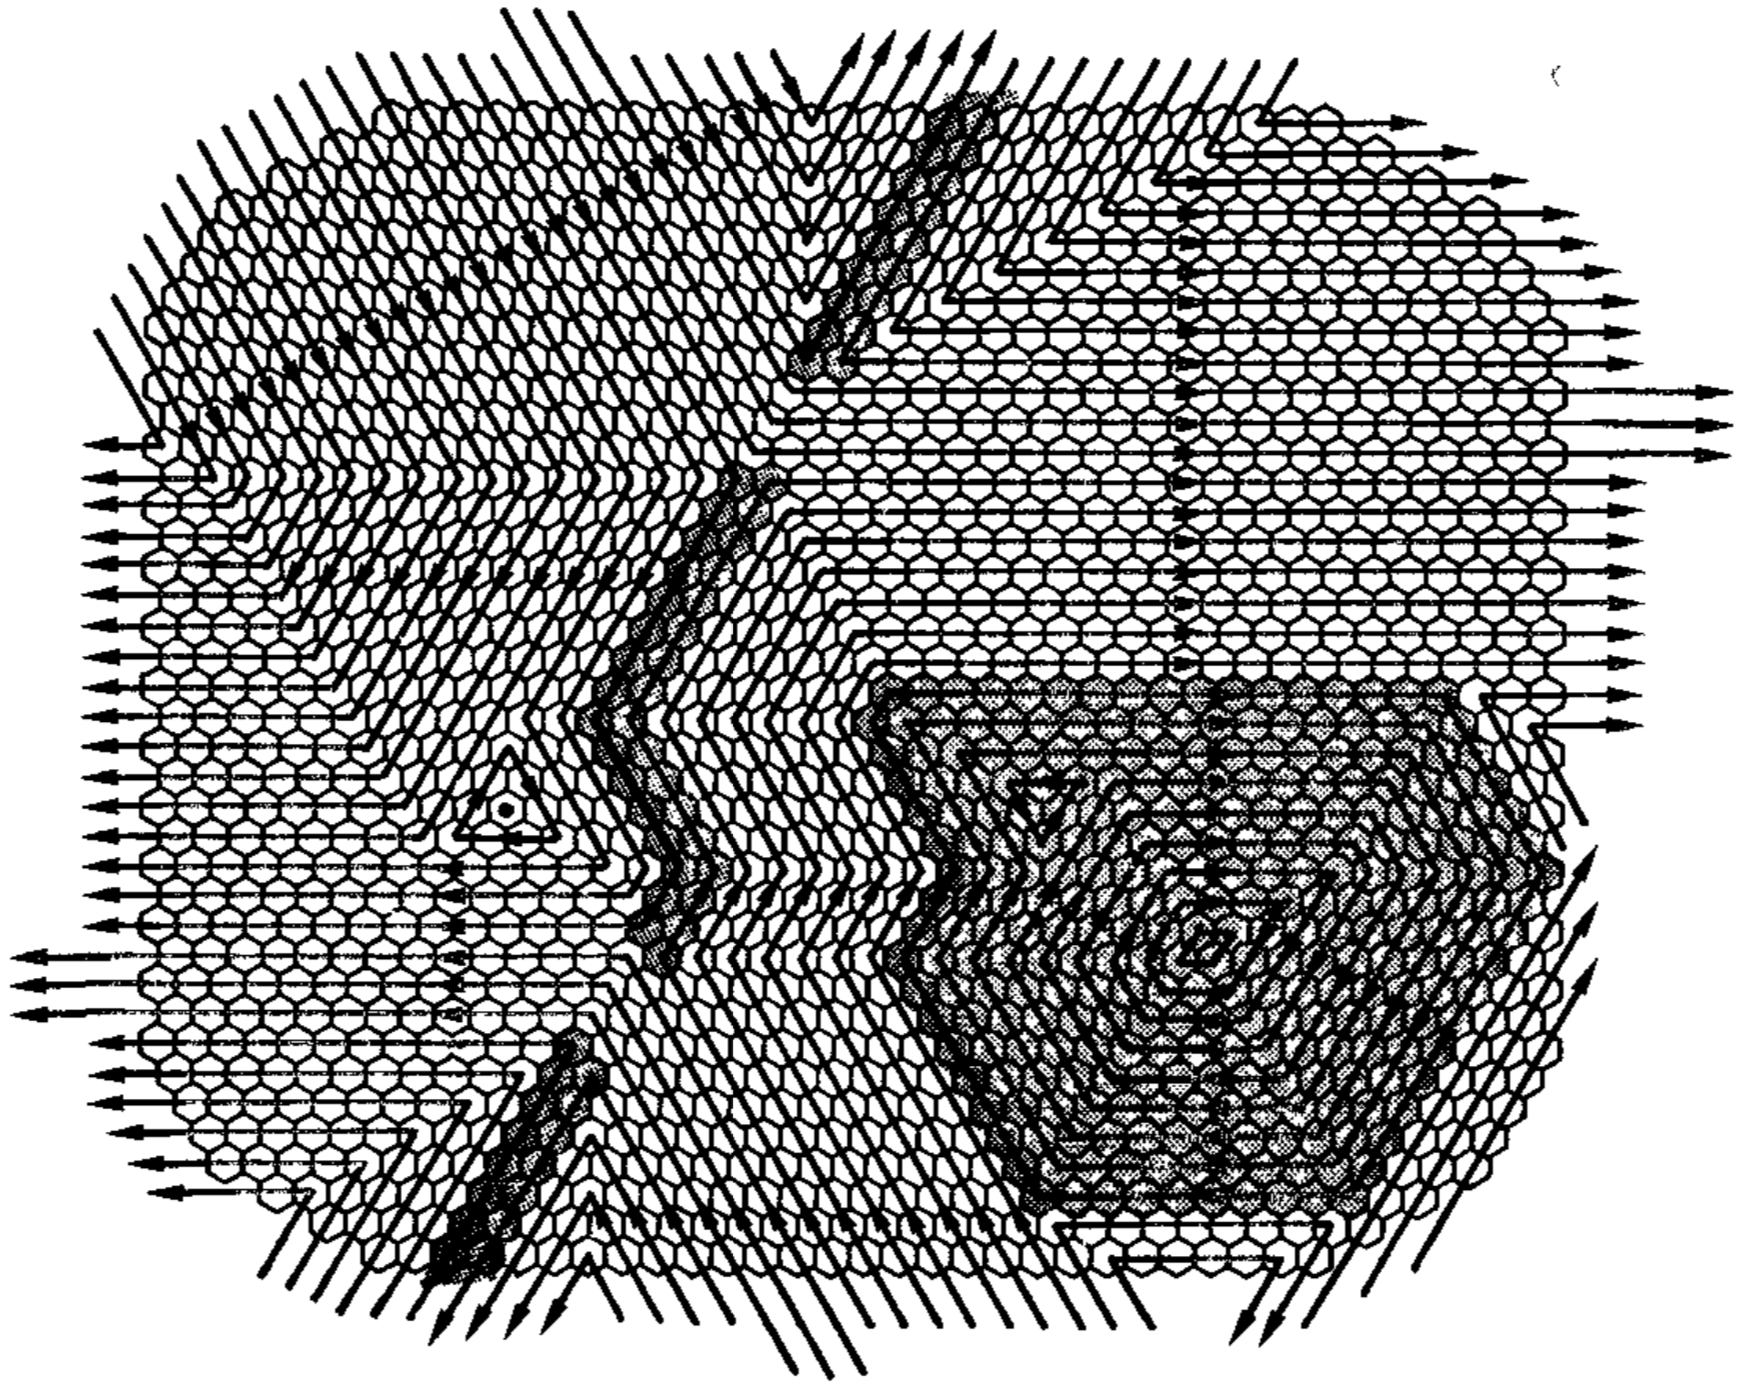
\includegraphics[width=0.8\textwidth]{phase_space.png}
    
    \footnotesize{\caption{A schematic representation of phase space. The hexagonal cells represent state points $( \bold{r}^N, \, \bold{p}^N )$. In an ergodic system, all the trajectories here would be different sections of a single long trajectory. Indeed, if the system is ergodic, the single long trajectory would eventually pass through (or arbitrarily near) all states. A substantial region of cyclical trajectories, and a barrier region leading to bottleneck, are shaded. 
    \textit{Source:} Allen and Tildesley, \textit{Computer Simulation of Liquids} (1st edition, 1987) 
    \cite{ref:AllenTildesley_1ed}.}
    \label{fig:generation-of-microcan_state}
    }
\end{minipage} 
\end{figure}

Given an ergodic trajectory, microcanonical phase space averages can be replaced by time averages over the trajectory according to:
\begin{equation}\label{eq:stat_mean_val}
\left< A \right> \:\equiv\: 
\frac{\int dx \; A(x) \: \delta(H (x) - E)}{\int dx \; \delta(H (x) - E)} \:=\: 
\lim_{\tau \rightarrow \infty} \; \frac{1}{\tau} \: \int_0^\tau dt \; A[x(t)] \:\equiv\: \bar{A}
\end{equation}
where $x(t)$ is a representative point of the phase space define as $x(t) \:=\: ( \bold{r}^N(t), \, \bold{p}^N(t) )$. 
This formula can be discretized for MD simulations as follow:
\begin{equation}\label{eq:stat_mean_val-discr}
\left< A \right> \:=\: \frac{1}{M} \: \sum_{n = 0}^M \: A(x_{n \, \Delta t})
\end{equation}

The discretization derive from the fact that the equations of motion are solved numerically using some numerical integrators that generate phase space vectors at discrete times that are multiples of a fundamental time discretization parameter $\Delta t$, known as \textit{the time step}.
Starting from $x_0$, the vectors $x_{n \, \Delta t}$ (where $n \:=\: 0 \, , \, \dots \, , \, M\:$ with $M$ as the total number of integration steps) are generated by applying the integrator iteratively\footnote{For biological MD simulations $\Delta t$ is usually of the order of few femtoseconds $(10^{-15} \: s)$ therefore, in order to obtain a trajectory of few nanoseconds $(10^{-9} \: s)$, one has to perform at least a million of integration steps.} \cite{ref:mypresentation}.
\begin{equation}\label{eq:discretization}
x(t) \xrightarrow[\quad t \;\rightarrow\; n\,\Delta t \quad]{} x_{n \, \Delta t}
\end{equation}

By the way, adopting classical point of view, doing a MD simulation basically means solving Newton's equations of motion for a system of $N$ interacting atoms: 
\begin{equation}\label{eq:newtons2law}
m_i \, \ddot{\bold{r}}_i \: = \: \bold{F}_i [\bold{r}^N(t)]
\qquad\qquad i \:=\: 1 \, , \, \dots \, , \, N
\end{equation}
where the forces are derived as the negative derivatives of the potential energy function $U [\bold{r}^N(t)]$:
\begin{equation}\label{eq:force-enpot}
\bold{F}_i [\bold{r}^N(t)] \:=\: - \, \nabla_{\bold{r}_i} \: U [\bold{r}^N(t)] 
\end{equation}
This equations are solved simultaneously every time steps. The system is followed for sometime, taking care that the temperature and pressure remain at the required values and the coordinates are written to an output file at regular intervals. The coordinates as a function of time represent a trajectory of the system. After initial changes, the system will usually reach an equillibrium state. By averaging over an equilibrium trajectory many macroscopic properties can be extracted from an output file.

%\section[Approaching to a real MD simulation: \textit{Setting up and running molecular dynamics simulations}]{Approaching to a real MD simulation\\ {\large \textit{Setting up and running molecular dynamics simulations}}}
\section{Molecular dynamics: concepts and algorithms}

In this section are shown several concepts that are useful to understand how MD simulations of macromolecular systems, like protein, generally work. Specifically, first it is introduce the problem of the calculation of the forces: classical MD force field and boundary condition with a considerations of the special case of the long range Coulomb interactions are shown. Then, there is a brief introduction to the numerical integration used to solve \eqref{eq:newtons2law} with an outline of simulation strategies for controlling temperature and pressure. Finally, the problem concerning the creation of the initial state is discussed: the starting structure, solvation, minimization and equilibration.

Note: these topics are presented focusing on a particular case of MD simulations - those concerning biological system and performed with NAMD software (see section ..). 
%Preparation of the system (i.e. creation of the initial state - $\bold{r}^N(t=0)$), 
%In the case of such simulationsintegration methods along with the efficient electrostatics evaluation algorithms employed and temperature and pressure controls used. 

%Below we introduce first the functional form of the force field utilized in NAMD. We then comment on the special problem of calculating the Coulomb potential and forces efficiently. The numerical integration of \eqref{eq:newtons2law} is then explained, followed by an outline of simulation strategies for controlling temperature. In the case of such simulations, frictional and fluctuating forces are added to \eqref{eq:newtons2law} following the principles of nonequilibrium statistical mechanics.

\subsection{Calculation of the forces}
The potential energy is one of the most crucial part of the simulation because it must faithfully represent the interaction between atoms, yet be cast in the form of a simple mathematical function that can be calculated quickly. Indeed the computation of the forces acting on every particle is the most time-consuming part of almost all MD simulations.

Hence, since biological systems involve many atoms of different types, a quantum mechanical treatment of these atoms is not feasible. The usual way to solve them is to use empirical potential energy functions, conventionally called \textit{force fields}, which are computationally less expensive, but involve numerous approximations leading to certain limitations.\footnote{A force field, in the context of a computer simulation, refers to the functional forms used to describe the intra-molecular and inter-molecular potential energy of a collection of atoms, and the corresponding parameters that will determine the energy of a given configuration. Thus it is a special case of interatomic potentials and it must not be confused with force field in classical physics.} 
These functions and parameters have been derived from experimental results and quantum mechanical calculations of small model compounds. They are often refined by the use of computer simulations to compare calculated condensed phase properties with experiment.
Current generation force fields provide a reasonable good compromise between accuracy and computational efficiency. 
Among the most commonly used potential energy functions are the AMBER, CHARMM, GROMOS and OPLS/AMBER force fields. However, one of the most important limitation of the empirical force fields is that no drastic changes in the electronic structure are allowed. i.e. no events like bond making or breaking can be modeled \cite{ref:MDsim_Gkeka}.

NAMD is able to use the parameterizations from both CHARMM and AMBER force field specifications.

%In approaching the simulation of a complicated system, there might be 30 different atom types to consider and several hundred different intra- and inter-molecular potentials to fit. One would probably not want to build the potential model from scratch, but the force is the most computationally demanding part of molecular dynamics. Fortunately, it is possible to draw on the considerable body of work that has gone into the development of consistent force fields over the last 50 years.
%
%There are several types of these force fields:
%\begin{itemize}
%\item[$\rhd$] \textbf{All-atom force fields:} provide parameters for every type of atom in a system, including hydrogen.
%\item[$\rhd$] \textbf{United-atom interatomic potentials:} treat the hydrogen and carbon atoms in each methyl group and each methylene bridge as one interaction center.
%\item[$\rhd$] \textbf{Coarse-grained potentials:} provide even cruder representations for higher computing efficiency. For this reason, they are often used in long-time simulations of macromolecules such as proteins, nucleic acids, and multi-component complexes.
%\end{itemize}

\subsubsection{Force field example: CHARMM}

As shown in eq. \eqref{eq:force-enpot}, the force acting on an atom $i$ is calculated as the negative gradient of a scalar potential energy function $U$ that that depends on all atomic positions and, thereby, couples the motion of atoms. For systems of biomolecules, this potential energy function is usually divided in two parts:
\begin{equation}\label{eq:forcefield-PotEnergy}
U \: = \: U_{\text{bonded}} \, + \, U_{\text{non-bonded}} 
\end{equation}

The bonded potential $U_{\text{bonded}}$ involve 2 , 3, and 4-body interactions of covalently bonded atoms, with $O(N)$ terms in the summation.\footnote{Indeed, the number of covalent bound is proportional to the number of atoms.}
The non-bonded potential $U_{\text{non-bonded}}$ involve long-range interactions between all pairs of atoms (usually excluding pairs of atoms already involved in a bonded term), with $O(N^2)$ terms in the summation, although fast evaluation techniques are used to compute good approximations to their contribution to the potential with $O(N)$ or $O(N$ log $N )$ computational cost. The different terms will now be presented in more detail.

\vspace{0.25cm}

\begin{center}
{\textbf{\textit{Bonded potential terms}}}
\end{center}
The bonded potential describe the stretching, bending, and torsional of the covalent bonds. 

\begin{figure}[H]
\centering
\begin{minipage}[t]{0.725\textwidth}
	\centering
    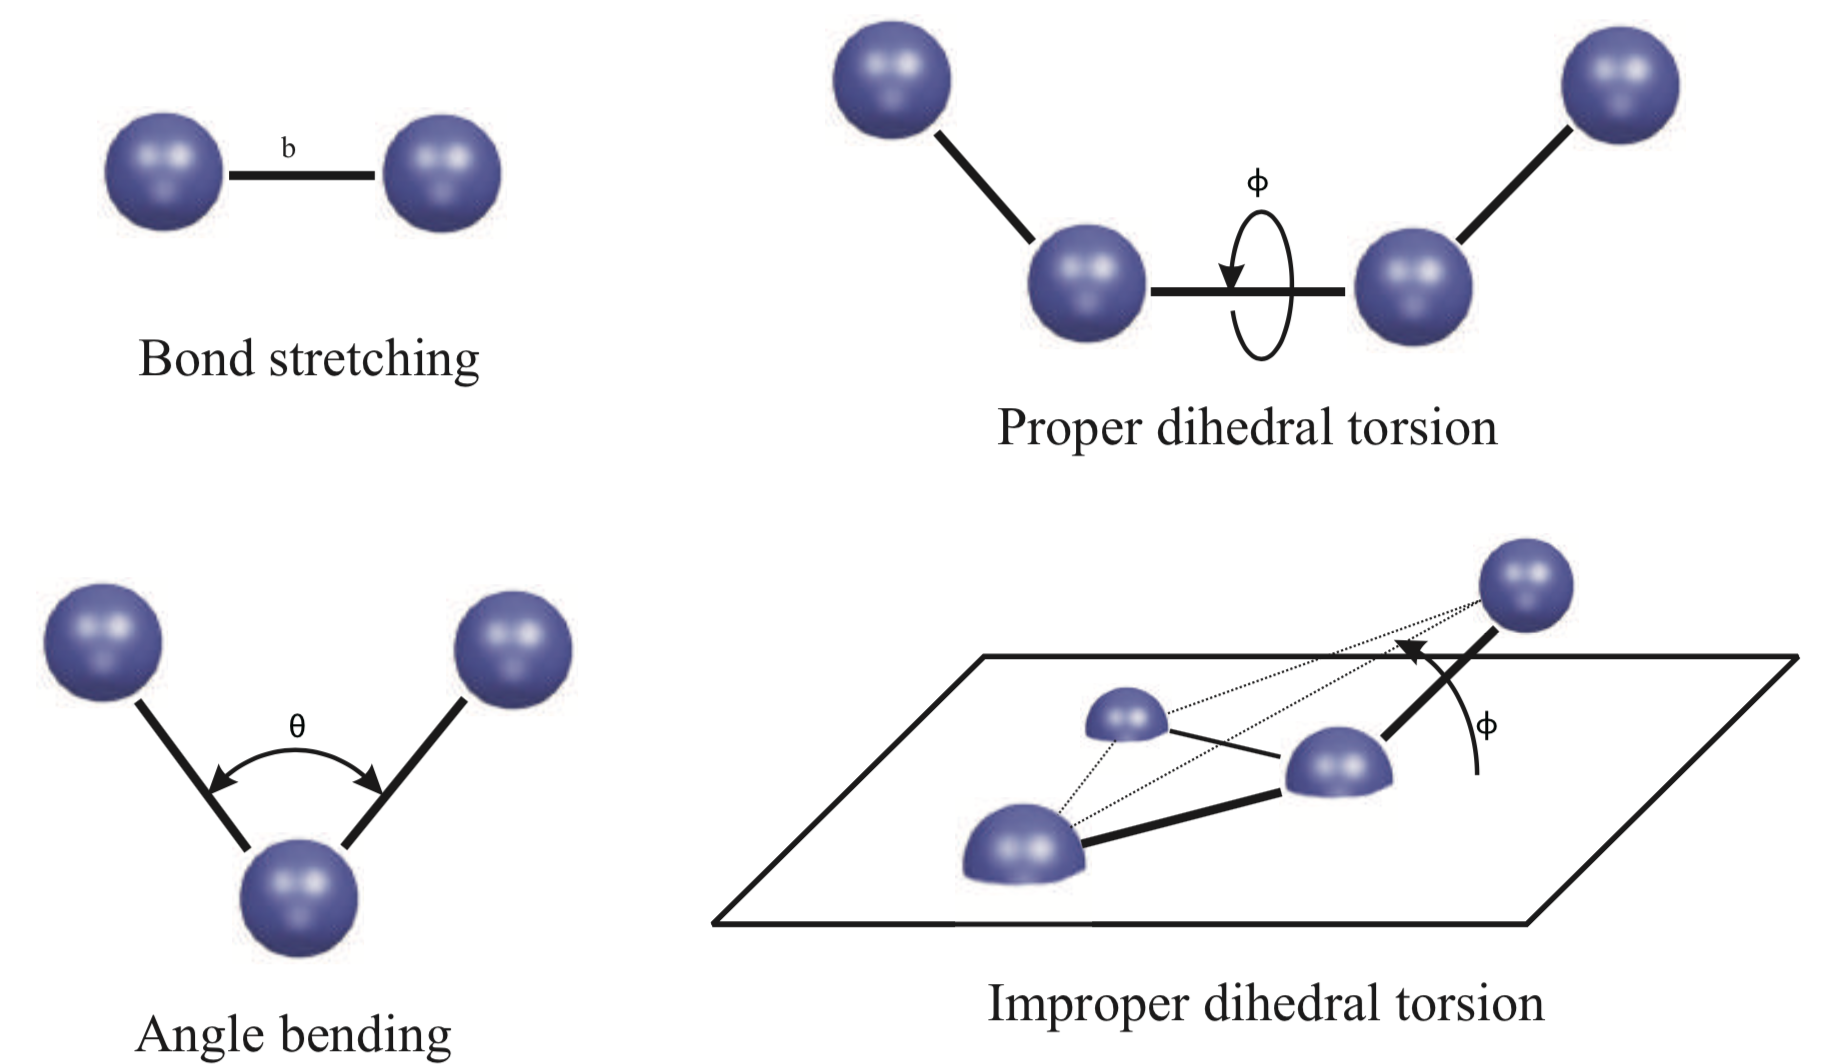
\includegraphics[width=0.7\textwidth]{bounded_interactions.png}
    
    \footnotesize{\caption{Schematic representation of the bonded interaction terms contributing to the force field.
    %: bond stretching, angle bending, proper and improper dihedrals.
    \textit{Source:} P. Gkeka and Z. Cournia, \textit{Molecular Dynamics simulations of lysozyme in water} (2015) 
    \cite{ref:MDsim_Gkeka}.}
    \label{fig:bounded_int}
    }
\end{minipage} 
\end{figure}

\begin{itemize}
\item[$\blacktriangleright$] \textbf{Bond stretching:}\\
The bond stretching term is a 2-body potential, generally assumed to be harmonic, that describes the vibrational motion between an pair of covalently bonded atoms:
\begin{equation}\label{eq:poten-bond_int}
U_b \: = \: k_b \: (b \,-\, b_0)^2
\end{equation}
where $b$ is the distance between the two atoms. Two parameters characterize each bonded
interaction: $b_0$ the average distance between them and a force constant $k_b$.

\item[$\blacktriangleright$] \textbf{Angle bending:}\\
The angle bending terms describes the force originating from the deformation of the valence angles between three covalently bonded atoms (3-body interactions). The angle bending term is described using a harmonic potential:
\begin{equation}\label{eq:poten-angle_int}
U_\theta \: = \: k_\theta \: (\theta \,-\, \theta_0)^2
\end{equation}
where $\theta$ is the angle between three atoms. There again two parameters characterize each
angle in the system: the reference angle $\theta_0$ and a force constant $k_\theta$. \\

\item[$\blacktriangleright$] \textbf{Torsional terms:}\\
The torsional terms are weaker than the bond stretching and angle bending terms. They describe the barriers to rotations existing between four bonded atoms (4-body interaction). There are two type of torsional terms: proper and improper dihedrals. Proper torsional potentials are described by a cosine function:
\begin{equation}\label{eq:poten-dihedral_int}
U_\phi \: = \: k_\phi \: [1 \, + \, \cos (n \, \phi \,-\, \delta)]
\end{equation}
where $\phi$ is the angle between the planes formed by the first and the last three of the four atoms. Three parameters characterize this interaction: $\delta$ sets the minimum energy angle, $k_\phi$ is a force constant and $n$ is the periodicity.

The improper dihedral term is designed both to maintain chirality about a tetrahedral heavy atom and to maintain planarity about certain atoms. The potential is described by a harmonic function:
\begin{equation}\label{eq:poten-imp_dihedral_int}
U_\omega \: = \: k_\omega \: (\omega \,-\, \omega_0)^2
\end{equation}
where $\omega$ is the angle between the plane formed by the central atom and two peripheral atoms and the plane formed by the peripheral atoms (see Fig. \ref{fig:bounded_int}).
\end{itemize}

\vspace{0.25cm}

\begin{center}
{\textbf{\textit{Non-bonded potential terms}}}
\end{center}
The non-bonded potential describes the van der Waals forces and the electrostatic interactions between the atoms. %These are non-bonded interactions, i.e., they act between atoms which are not covalently bonded together.

\begin{figure}[H]
\centering
\begin{minipage}[t]{0.68\textwidth}
	\centering
    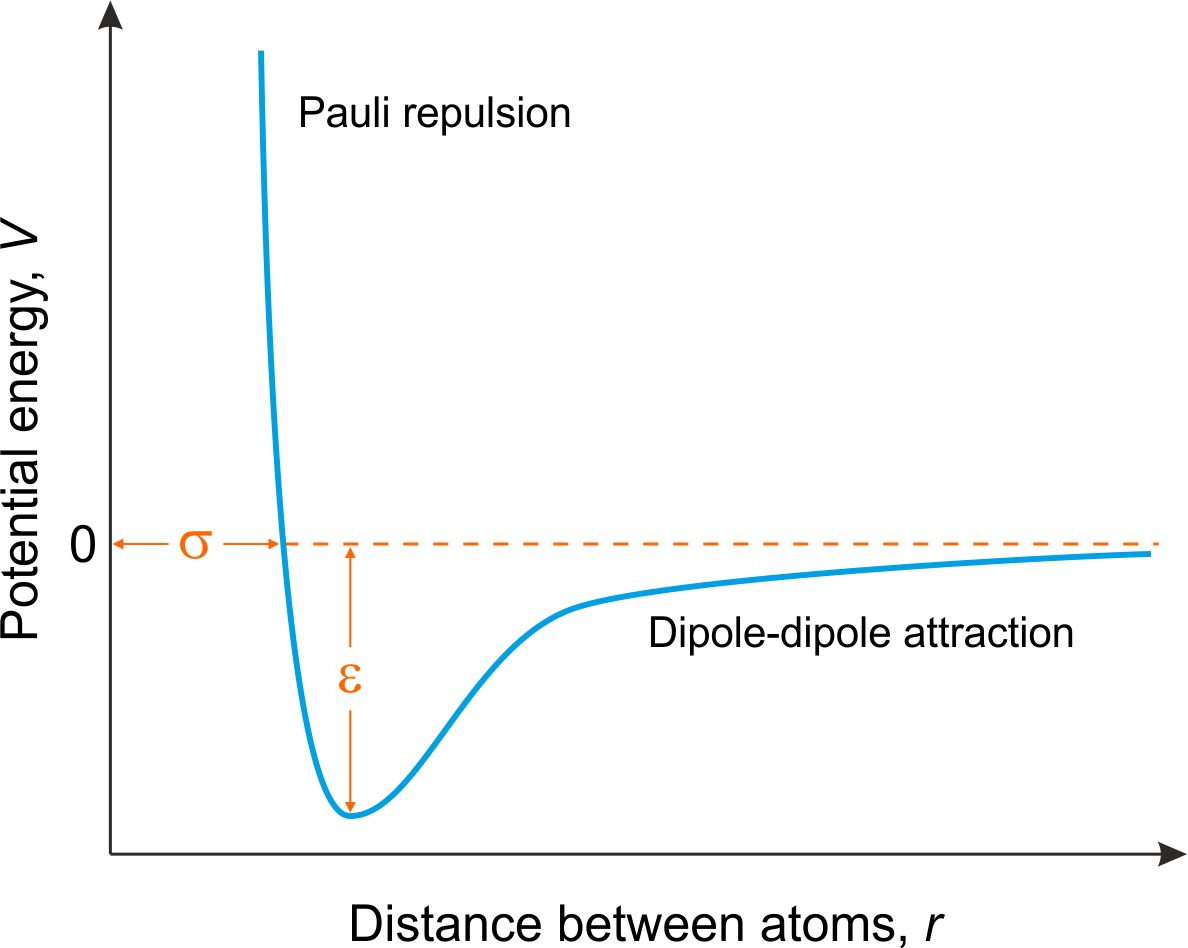
\includegraphics[width=0.65\textwidth]{lennard-jones_potential.png}
    
    \footnotesize{\caption{Schematic representation of Lennard-Jones potential. The collision parameter, $\sigma$, is shown along with the well depth, $\epsilon$.
    \textit{Source:} Eni. Generalic, \textit{Lennard-Jones potential} (Croatian-English Chemistry Dictionary \& Glossar, 2017) 
    \cite{ref:LJpot-graph}.}
    \label{fig:bounded_int}
    }
\end{minipage} 
\end{figure}

\begin{itemize}
\item[$\blacktriangleright$] \textbf{Van der Waals interactions:}\\
The van der Waals force acts on atoms in close proximity. It is strongly repulsive at short range and weakly attractive at medium range. The interaction is described by a Lennard-Jones potential:
\begin{equation}\label{eq:LJpotential}
U_{VdW} \: = \: 4 \, \epsilon \: \left[ \left(\frac{\sigma}{r}\right)^{12} \,-\; \left(\frac{\sigma}{r}\right)^6 \right]
\end{equation}
where $r$ is the distance between two atoms. It is parameterized by $\sigma$: the collision parameter (the separation for which the energy is zero) and $\epsilon$ the depth of the potential well.
 The Lennard–Jones potential approaches 0 rapidly as $r$ increases, so it is usually truncated (smoothly shifted) to 0 past a cutoff radius, requiring $O(N)$ computational cost.

\item[$\blacktriangleright$] \textbf{Electrostatic interactions:}\\
Finally, the long distance electrostatic interaction between two atoms is described by Coulomb's law:
\begin{equation}\label{eq:Coulomb_potential}
U_{el} \: = \: \epsilon_{1-4} \: \cdot \: \frac{q_1 \: q_2}{4 \, \pi \, \epsilon_0 \: r_{12}}
\end{equation}
where $q_1$ and $q_2$ are the charges of both atoms and $r_{12}$ the distance between them, while $\epsilon_0$ is the electric susceptibility of vacuum.
The parameter $\epsilon_{1-4}$ is a unitless scaling factor whose value is 1, except for a modified $1-4$ interaction, where the pair of atoms is separated by a sequence of three covalent bonds (so that the atoms might also be involved in a torsion angle interaction), in which case $\epsilon_{1-4} \:=\: \epsilon$, for a fixed constant $0 \leq \epsilon \leq 1$. 
Although the electrostatic potential may be computed with a cutoff like the Lennard-Jones potential, the $r^{-1}$ potential approaches 0 much more slowly than the $r^{-6}$ potential, so neglecting the long range electrostatic terms can degrade qualitative results, especially for highly charged systems. There are other fast evaluation methods that approximate the contribution to the long range electrostatic terms that require $O(N)$ or $O(N \log N)$ computational cost, depending on the method.
\end{itemize}

\vspace{0.25cm}

\begin{center}
{\textbf{\textit{Potential energy function}}}
\end{center}
So finally, the equation for the potential energy describing the force field can be written:
\begin{subequations}\label{eq:ForceField}
\begin{equation}\label{eq:ForceField-bonded}
\left.
	\begin{array}{ll} 
	U \;&=\; \mathlarger{\sum}\limits_{bonds \: b} \: k_b \: (b \,-\, b_0)^2 
	\;+\; \mathlarger{\sum}\limits_{angles \, \theta} \: k_\theta \: (\theta \,-\, \theta_0)^2\;+\\
	&\vspace{0.1cm}\\
	&+\; \mathlarger{\sum}\limits_{\substack{proper \\ dihedrals}} \: k_\phi \: 
	[1 \, + \, \cos (n \, \phi \,-\, \delta)]
	\;+\; \mathlarger{\sum}\limits_{\substack{improper \\ dihedrals}} \: k_\omega \: 
	(\omega \,-\, \omega_0)^2\;+\\
	\end{array}
\;\right\}\;\substack{\text{\textsc{\textbf{Bonded}}}\\ \text{\textsc{\textbf{interactions}}}}
\end{equation}

\vspace{-0.5cm}

\begin{equation}\label{eq:ForceField-nonbonded}
	\qquad\quad+\;\; \mathlarger{\sum}\limits_{\substack{i, \, j\\j<i}} \: 4 \, \epsilon \: \left[ \left(\frac{\sigma}{r}\right)^{12} \,-\; \left(\frac{\sigma}{r}\right)^6 \right]
	+\; \mathlarger{\sum}\limits_{\substack{i, \, j\\j<i}} \: \epsilon_{1-4} \: \cdot \: \frac{q_1 \: q_2}{4 \, \pi \, \epsilon_0 \: r_{12}}
\qquad\Longrightarrow\quad\substack{\text{\textsc{\textbf{Non-bonded}}}\\ \text{\textsc{\textbf{interactions}}}}
\end{equation}
\end{subequations}
%\begin{equation}
%\begin{split}
%U \;&=\; 
%\sum_{bonds \: b} \: k_b \: (b \,-\, b_0)^2 \;+\; \sum_{angles \, \theta} \: k_\theta \: (\theta \,-\, \theta_0)^2\\
%&+\; \sum_{\substack{proper \\ dihedrals}} \: k_\phi \: [1 \, + \, \cos (n \, \phi \,-\, \delta)] \;+\; \sum_{\substack{improper \\ dihedrals}} \: k_\omega \: (\omega \,-\, \omega_0)^2\\
%&+\; \sum_{\substack{i, \, j\\j<i}} \: 4 \, \epsilon \: \left[ \left(\frac{\sigma}{r}\right)^{12} \,-\; \left(\frac{\sigma}{r}\right)^6 \right] \;+\;
%\sum_{\substack{i, \, j\\j<i}} \: \epsilon_{1-4} \: \cdot \: \frac{q_1 \: q_2}{4 \, \pi \, \epsilon_0 \: r_{12}}
%\end{split}
%\end{equation}

\vspace{0.25cm}

\subsubsection{Boundary condition}
To avoid surface effects at the boundary of the simulated system, periodic boundary conditions are often used in MD simulations; the particles are enclosed in a cell that is replicated to infinity by periodic translations. A particle that leaves the cell on one side is replaced by a copy entering the cell on the opposite side, and each particle is subject to the potential from all other particles in the system including images in the surrounding cells, thus entirely eliminating surface effects (but not finite-size effects). Because every cell is an identical copy of all the others, all the image particles move together and need only be represented once inside the molecular dynamics code.
\begin{figure}[H]
\centering
\begin{minipage}[t]{0.75\textwidth}
	\centering
    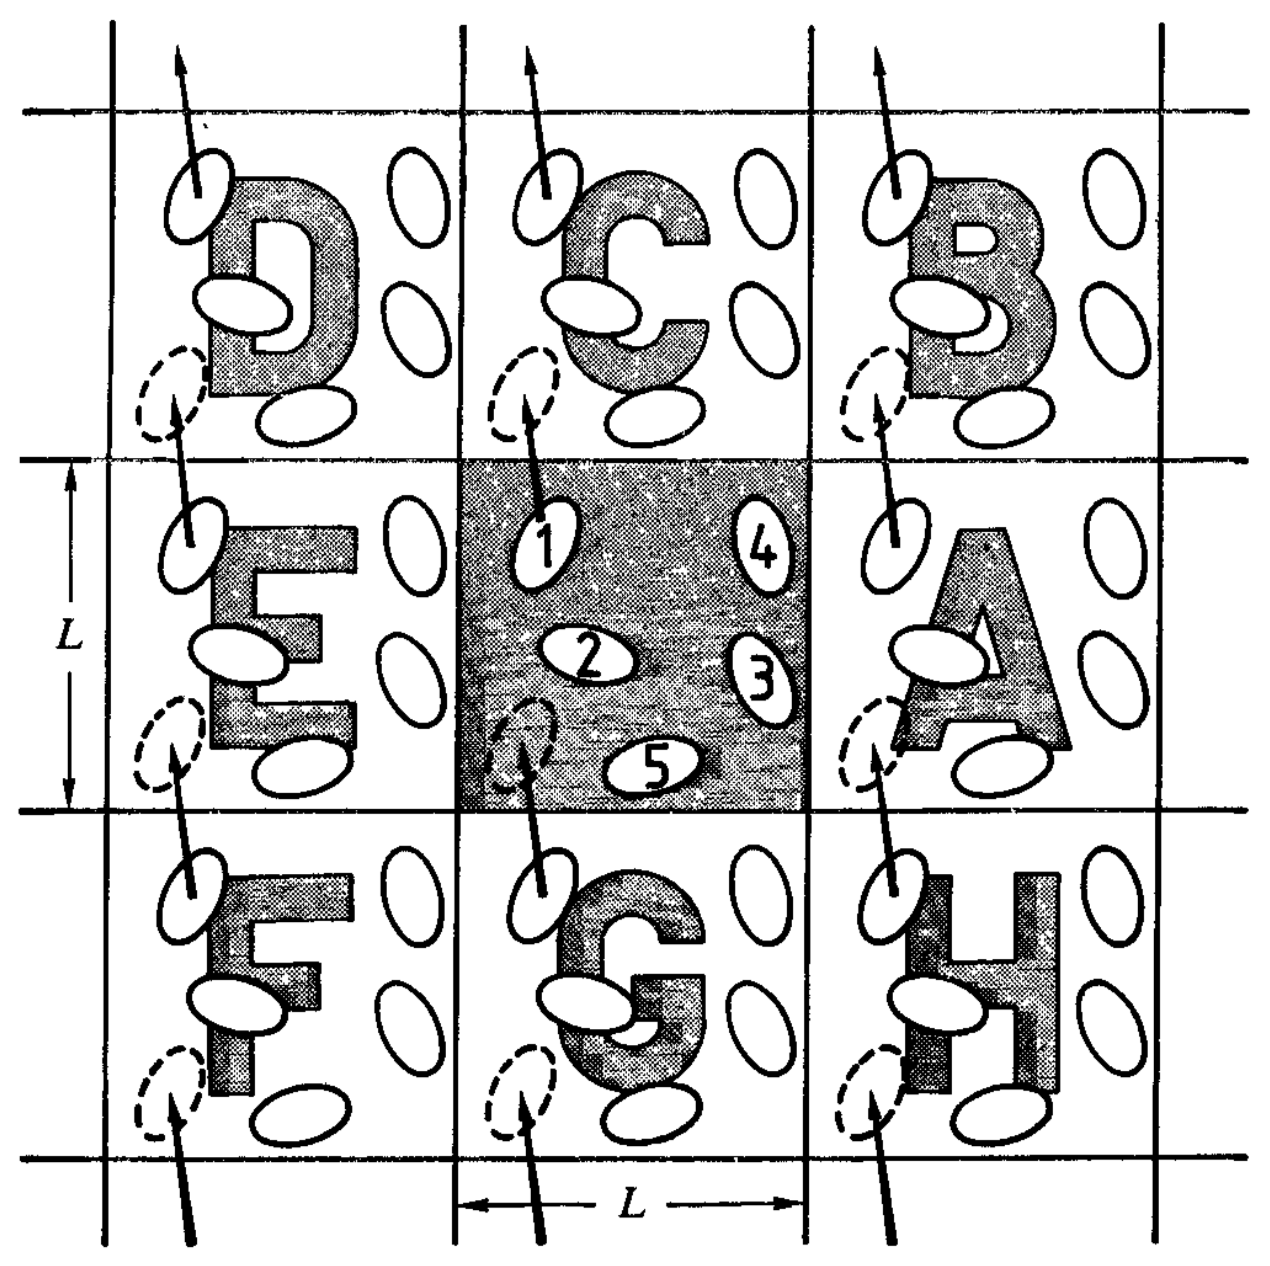
\includegraphics[width=0.45\textwidth]{periodic_cond.png}
    
    \footnotesize{\caption{A two-dimensional periodic system. Molecules can enter and leave each box across each of the four edges. In a three-dimensional example, molecules would be free to cross any of the six cube faces.
    \textit{Source:} Allen and Tildesley, \textit{Computer Simulation of Liquids} (1st edition, 1987) 
    \cite{ref:AllenTildesley_1ed}.}
    \label{fig:PME}
    }
\end{minipage} 
\end{figure}


However, because the van der Waals and electrostatic interactions exist between every nonbonded pair of atoms in the system (including those in neighboring cells) computing the long-range interaction exactly is unfeasible. To perform this computation, the van der Waals interaction is spatially truncated at a user-specified cutoff distance. For a simulation using periodic boundary conditions, the system periodicity is exploited to compute the full (nontruncated) electrostatic interaction with minimal additional cost using the particle-mesh Ewald (PME) method described in the next paragraph.

\vspace{0.25cm}

\begin{center}
{\textbf{\textit{Full Electrostatic Computation}}}
\end{center}
Ewald summation is a description of the long-range electrostatic interactions for a spatially limited system with periodic boundary conditions. The infinite sum of charge-charge interactions for a charge-neutral system is conditionally convergent, meaning that the result of the summation depends on the order in which it is taken. Ewald summation specifies the order as follows: sum over each box first, then sum over spheres of boxes of increasingly larger radii. Ewald summation is considered more reliable than a cutoff scheme, although it is noted that the artificial periodicity can lead to bias in free energy, and can artificially stabilize a protein that should have unfolded quickly.

The particle-mesh Ewald (PME) method is a fast numerical method to compute the Ewald sum. The cost of PME is proportional to $N \log N$ and the time reduction is significant even for a small system of several hundred atoms. 
The strict conservation of energy resulting from the computed force is crucial and is strongly assisted by maintaining the symplecticness of the integrator, as discussed further below.
However the PME method does not conserve energy and momentum simultaneously, but momentum conservation can be enforced by subtracting the net force from the reciprocal sum computation, albeit at the cost of a small long-time energy drift.

\begin{figure}[H]
\centering
\begin{minipage}[t]{0.8\textwidth}
	\centering
    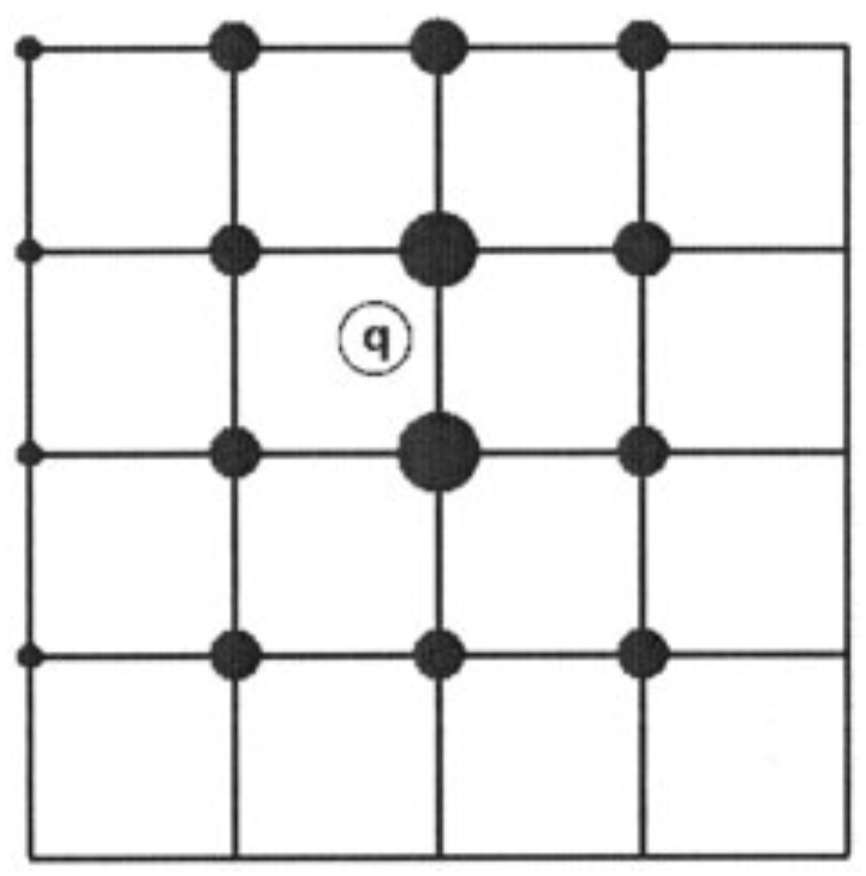
\includegraphics[width=0.325\textwidth]{PME.png}
    
    \footnotesize{\caption{In PME, a charge (denoted by an empty circle with label \textbf{q} in the figure) is distributed over grid (here a mesh in two dimensions) points with weighting functions chosen according to the distance of the respective grid points to the location of the charge. Positioning all charges on a grid enables the application of the FFT method and significantly reduces the computation time. In real applications, the grid is three-dimensional.
    \textit{Source:} J. C. Phillips et al., \textit{Scalable Molecular Dynamics with NAMD} (Journal of Computational Chemistry, 2005) 
    \cite{ref:NAMD}.}
    \label{fig:PME}
    }
\end{minipage} 
\end{figure}

\subsection{Numerical Integration}
Biomolecular simulations often require millions of time steps. Furthermore, biological systems are chaotic; trajectories starting from slightly different initial conditions diverge exponentially fast and after a few picoseconds are completely uncorrelated. However, highly accurate trajectories is not normally a goal for biomolecular simulations; more important is a proper sampling of phase space. Therefore, for constant energy (NVE ensemble) simulations, the key features of an integrator are not only how accurate it is locally, but also how efficient it is, and how well it preserves the fundamental dynamical properties, such as energy, momentum, time-reversibility, and symplecticness.

\begin{figure}[H]
\centering
\begin{minipage}[t]{0.8\textwidth}
	\centering
    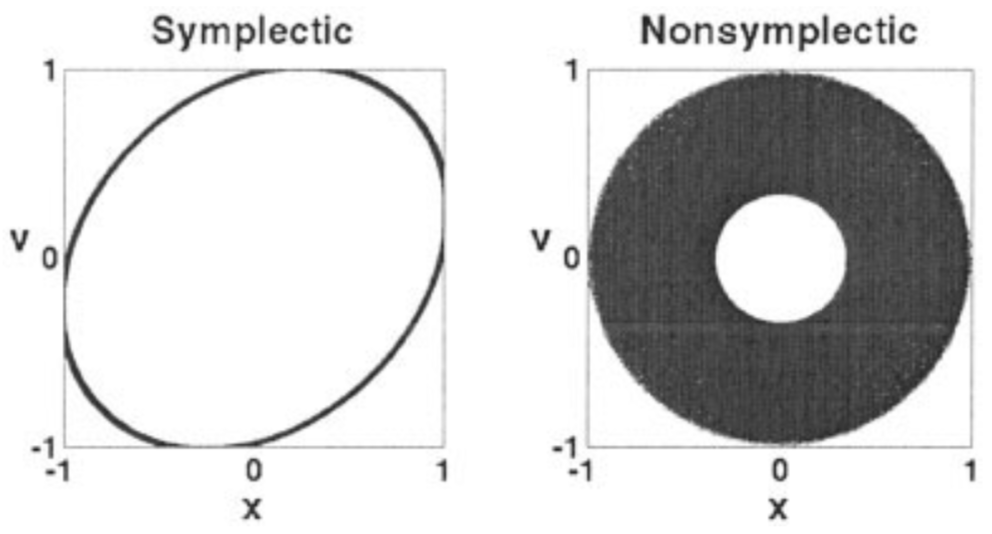
\includegraphics[width=0.6\textwidth]{symplettic_integrator.png}
    
    \footnotesize{\caption{Simple example that shows the merit of a symplectic integrator: integration of a one-dimensional harmonic oscillator with an unit circle as exact trajectory. The trajectory of nonsymplectic method initially draw a circle, but after few steps starts to collapse toward the center while the symplectic method maintains a stable orbit, showing a superior long-time stability, even though its trajectory is deformed into an ellipse by a larger local error.
    \textit{Source:} J. C. Phillips et al., \textit{Scalable Molecular Dynamics with NAMD} (Journal of Computational Chemistry, 2005) 
    \cite{ref:NAMD}.}
    \label{fig:symplettic-integrator}
    }
\end{minipage} 
\end{figure}

The time evolution of a strict Hamiltonian system is symplectic. A consequence of this is the conservation of phase space volume along the trajectory, that is, the enforcement of the Liouville theorem. To a large extent, the trajectories computed by numerical integrators observing symplecticness represent the solution of a closely related problem that is still Hamiltonian. Because of this, the errors, unavoidably generated by an integrator at each time step, accumulate imperceptibly slowly, resulting in a very small long-time energy drift, if there is any at all. Artificial measures to conserve energy, for example, scaling the velocity at each time step so that the total energy is constant, lead to biased phase space sampling of the constant energy surface; in contrast, there has been no evidence that symplectic integrators have this problem.

NAMD uses the velocity Verlet method for NVE ensemble simulations. This  method obtains the position and velocity at the next time step $( r_{n+1} , \, v_{n+1} )$ from the current one $( r_{n} , \, v_{n} )$, assuming the force $F_n \:=\: F(r_n)$ is already computed, in the following way:
\begin{equation*}
\begin{array}{rrcl}
\vspace{0.15cm}
\text{\textit{half-kick  }} \rightarrow &
v_{n + \frac{1}{2}} &= &v_n \,+\, 0.5 \cdot \Delta t \cdot F_n / m\\

\vspace{0.15cm}
\text{\textit{drift  }} \rightarrow& 
r_{n + 1} &= &r_n \,+\, \Delta t \cdot v_{n + \frac{1}{2}}\\

\vspace{0.15cm}
\text{\textit{compute force  }} \rightarrow&
F_{n+1} &= &F(r_{n+1})\\

\vspace{0.15cm}
\text{\textit{half-kick  }} \rightarrow& 
v_{n + 1} &= &v_{n + \frac{1}{2}} \,+\, 0.5 \cdot \Delta t \cdot F_{n + 1} / m\\
\end{array}
\end{equation*}
where $m$ is the mass. The Verlet method is symplectic and time reversible, conserves linear and angular momentum, and requires only one force evaluation for each time step. For a fixed time period, the method exhibits a (global) error proportional to $\Delta t^2$.

\begin{figure}[H]
\centering
\begin{minipage}[t]{0.8\textwidth}
	\centering
    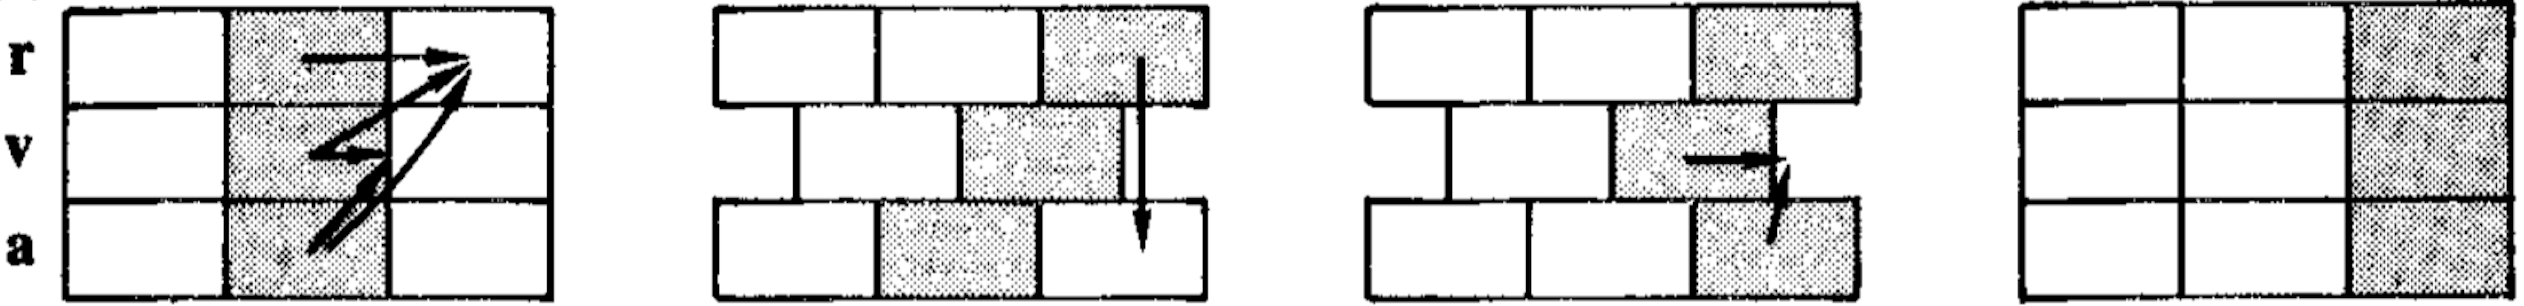
\includegraphics[width=0.9\textwidth]{VelocityVerlet-01.png}
    
    \footnotesize{\caption{Schematic representation of the velocity Verlet algorithm. At each steps, the stored variables are in grey boxes.
    \textit{Source:} Allen and Tildesley, \textit{Computer Simulation of Liquids} (1st edition, 1987) 
    \cite{ref:AllenTildesley_1ed}.}
    \label{fig:symplettic-integrator}
    }
\end{minipage} 
\end{figure}

More accurate (higher order) methods are desirable if they can increase the time step per force evaluation. However, higher order Runge-Kutta type methods, symplectic or not, are not suitable for biomolecular simulations because they require several force evaluations for each time step and force evaluation is by far the most time-consuming task in molecular dynamics simulations.
Gear type predictor-corrector methods, or linear multistep methods in general, are not symplectic. Hence, no symplectic method has been found as yet that is both more accurate than the Verlet method and as practical for biomolecular simulations.

NAMD employs a multiple-time-stepping method to improve integration efficiency. Because the biomolecular interactions collected in eq. \eqref{eq:ForceField} generally give rise to several different time scales characteristic for biomolecular dynamics, it is natural to compute the slower-varying forces less frequently than faster varying ones in molecular dynamics simulations. This idea is implemented in NAMD by three levels of integration loops. The inner loop uses only bonded forces to advance the system, the middle loop uses Lennard–Jones and short-range electrostatic forces, and the outer loop uses long-range electrostatic forces.\footnote{In the article: \textit{Scalable Molecular Dynamics with NAMD} (Journal of Computational Chemistry, 2005), Phillips and his colleagues note that the method implemented in NAMD is symplectic and time reversible \cite{ref:NAMD}.}

Using multiple time stepping can increase computational efficiency by a factor of 2, however the longest time step for the multiple time-stepping method is limited by resonance.\footnote{When good energy conservation is needed for NVE ensemble simulations Phillips and his colleagues recommend choosing $2 fs$, $2 fs$, and $4 fs$ as the inner, middle, and outer time steps if rigid bonds to hydrogen atoms are used; or $1 fs$, $1 fs$, and $3 fs$ if bonds to hydrogen are flexible. More aggressive time steps may be used for NVT or NPT ensemble simulations, for example, $2 fs$, $2 fs$, and $6 fs$ with rigid bonds and $1 fs$, $2 fs$, and $4 fs$ without \cite{ref:NAMD}.}

\subsection{NVT Ensemble Simulations}
A fundamental requirement for an integrator is to generate the correct ensemble distribution for the specified temperature and pressure in an appropriate way. For this purpose the Newtonian equations of motion \eqref{eq:newtons2law} should be modified ``mildly'' so that the computed short-time trajectory can still be interpreted in a conventional way. To generate the correct ensemble distribution, the system is coupled to a reservoir, with the coupling being either deterministic or stochastic. Deterministic couplings generally have some conserved quantities (similar to total energy), the monitoring of which can provide some confidence in the simulation. NAMD uses a stochastic coupling approach because it is easier to implement and the friction terms tend to enhance the dynamical stability.

The (stochastic) Langevin equation is used in NAMD to generate the Boltzmann distribution for canonical (NVT) ensemble simulations. The generic Langevin equation is:
\begin{equation}\label{eq:NVT-Langevin}
m_i \ddot{\bold{r}}_i(t) \:=\: \bold{F}_i[\bold{r}^N(t)] \,-\, \gamma \, \dot{\bold{r}}_i(t) \,+\, \sqrt{\frac{2 \, \gamma \, k_B T}{m_i}} \, \bold{R}(t)
\end{equation}
where $\gamma$ is the friction coefficient, $k_B$ is the Boltzmann constant, $T$ is the temperature and $\bold{R}(t)$ is a univariate Gaussian random process. Coupling to the reservoir is modeled by adding the fluctuating (the last term) and dissipative ($-\,  \gamma \: \dot{\bold{r}}_i $ term) forces to the Newtonian equations of motion. To integrate the Langevin equation, NAMD uses the Br\"{u}nger-Brooks-Karplus (BBK) method, a natural extension of the Verlet method for the Langevin equation. The position recurrence relation of the BBK method is:

\begin{equation}
r_{n+1} \;=\; r_n \:+\: \frac{1 \,-\, 0.5 \, \gamma \, \Delta t}{1 \,+\, 0.5 \, \gamma \, \Delta t} \: (r_n \,-\, r_{n-1}) \:+\: \frac{\Delta t^2}{1 \,+\, 0.5 \, \gamma \, \Delta t} \: \left[ \frac{F(r_n)}{m} \:+\: \sqrt{\frac{2\, \gamma \, k_B T}{m}} \: Z_n \right]
\end{equation}
where $Z_n$ is a set of Gaussian random variables of zero mean and variance 1. The BBK integrator requires only one random number for each degree of freedom. The steady-state distribution generated by the BBK method has an error proportional to $\Delta t^2$, although the error in the time correlation function can have an error proportional to $\Delta t$.

\subsection{Initial configuration of the system}
To begin a MD simulation, before to start with the integration of the equation of motion, it is necessary to choose  an initial configuration of the system, i.e. to set first the coordinates and the velocities of all the atoms. In particular, for simulations with biomolecules, due to the complex structures of these macromolecules, the initial positions of their atoms are usually obtained from the Protein Data Bank: a great repository of information about the 3D structures, drawn by the results of X-rays crystallography and NMR experiments,
%(drawn with X-rays crystallography and NMR measures) 
%(X-ray crystal structure or an NMR structure) 
of proteins, nucleic acids, and complex assemblies.
These sets of coordinates, representing macromolecular structures, are used as the starting point of these type simulations with the aim of getting, through several processes that modify these coordinates, an initial configuration of the entire system that it is as close as possible to the configuration of the real system that it is intended to study. When the initial configuration is achieved, it is possible to make several simulations of the system that can be used to measure some of its properties (this phase of the simulation is conventionally named: \textit{production phase} and the main scope of a molecular simulation is to get some interesting results from this phase). The process generally used in MD simulations of biological system, preceding the production phase, are mainly the follow: solvation, minimization, heating (set the velocities) and equilibration; that are describe below.

In any case, it is important to point out that the choice of the initial configuration must be done carefully as this can influence the quality of the entire simulation.

\subsubsection{Solvation}
Solvation consist in the process of tacking into account the solvent from which the biomolecules are surrounded. Actually, biomolecules are generally in solution with some types of aqueous solvent and therefore solvation is a common process that is used to prepare the initial configuration of the system. This is indeed due to the known fact that solvation effects play a crucial role in determining molecular conformation, electronic properties, binding energies, etc.

There are mainly two way to solvate a a biomolecular system:
\begin{itemize}
\item \textbf{explicit treatment:} the coordinates of the solvent atoms are directly added to the system with the specification of the structure of the molecules that occur in the solvent (most often water molecule and, sometimes, also salt ions also).\footnote{Usually, in this phase of the simulation, periodic boundary condition is particularly important to avoids surface effects.} 
\item \textbf{implicit treatment:} the force field is modified to include also the effect due to the interaction between the biomolecular system and the solvent. Thus this technique eliminates the need of specifying all the atoms of the solvent by including many of their average effects in the inter-atomic force calculation. For example, polar solvent acts as a dielectric and screens (lessens) electrostatic interactions. 
\end{itemize}

The elimination of explicit water accelerates conformational explorations and sometimes increases simulation speed, although at the cost of not modeling the solvent as accurately as explicit models.
Indeed the implicit solvent models eliminate explicit water molecules and represent water in an averaged manner, hence implicit solvent models are considered less accurate than explicit solvent models. Always caution should be used when implicit solvent are employed for molecular dynamics research.

\subsubsection{Minimization}
In the context of MD simulation, the energy minimization, or simply minimization, is the process of finding an arrangement in space for a collection of atoms where, according to the force field used, the net inter-atomic force on each atom is acceptably close to zero and the position on the potential energy surface is a stationary point. Generally speaking, the collection of atoms might be a single molecule, an ion, a condensed phase, a transition state or even a collection of any of these. 

As an example, when optimizing the geometry of a water molecule, one aims to obtain the hydrogen-oxygen bond lengths and the hydrogen-oxygen-hydrogen bond angle which minimize the forces that would otherwise be pulling atoms together or pushing them apart.

The motivation for performing a energy minimization is the physical significance of the obtained structure: even when initial coordinates are available from experiment, the starting vector may not correspond to a minimum in the potential energy function used, and hence minimization is needed to relax strained contacts. When an experimental structure is not available, a build-up technique may be used to construct a structure on the basis of the known building blocks, and minimization again is required.

For a biomolecular system, the potential energy function is a very complex and multidimensional landscape. It has one deepest point, the global minimum, and a very large number of local minima. The goal of the energy minimization is to find a local minimum. The energy at this local minimum may be much higher than the energy of the global minimum. Performing an energy minimization will guarantee the removal of any strong van der Waals interations that may exist which might otherwise lead to local structural distortion and result in an unstable simulation.


\subsubsection{Heating}

The initial velocities at low temperature are assigned to each atom of the system and Newton's equations of motion are integrated to propagate the system in time. During the heating phase, initial velocities are assigned at a low temperature and the simulation is started with periodically assigning new velocities at a slightly higher temperature and letting the simulation continue. This step is repeated until the desired temperature is reached.

Heating and cooling or equilibration at fixed temperature permits biopolymer to escape local minima
XX
The initial velocities of each atom of the system are typically set pseudorandomly so that the total kinetic energy of the system corresponds to the expected value at the target temperature $T$. According to the classical equipartition theorem, each normal mode has $k_B \, T \,/\,2$ energy, on average, at thermal equilibrium.

The heating process, usually done in the NVT ensemble, consist in the progressively increasing of  the reservoir's temperature to heat gradually the system. This process has mainly two different aims: 
\begin{itemize}
\item reach the desired temperature at which the system has to be studied;
\item change the configuration of the system with the purpose of escape from some local minima of the energy landscape that probably do not represent the real state of the system.\footnote{This might be done also in alternation with some phases of cooling.}
\item change the configuration of the system to escape from local minima of the energy landscape that probably are reached with the minimization but that do not represent the real state of the system.\footnote{This might be done also in alternation with some phases of cooling.}
\end{itemize}
In any case, the need of a gradually increase of the temperature is due to the fact that, starting from the structures obtained from the x-ray experiment, typically made at low temperature, and after some manipulations and the minimization that modify these structures, the configuration of the system obtained in this way is built without taking into account the velocities and hence the contribution of the kinetic energy to the total energy. Thus starting with an artificial configuration of the``frozen'' system 

At the beginning of the heating the velocities of the atoms are typically set pseudorandomly so that the total kinetic energy of the system corresponds to the expected value at the target temperature $T$.

Sometime, since the structures obtained from the x-ray experiment might be made at low temperature and because after the minimization, done with the system "frozen" without an the configuration of the system might correspond to a situation in which the kine, it is useful to start the simulation with velocities that correspond at temperature of the same order.
This initialization is typically made setting pseudorandomly so that the total kinetic energy of the system corresponds to the expected value at the target temperature $T$. According to the classical equipartition theorem, each normal mode has $k_B \, T \,/\,2$ energy, on average, at thermal equilibrium.

The initial velocities are typically set pseudorandomly so that the total kinetic energy of the system corresponds to the expected value at the target temperature $T$. According to the classical equipartition theorem, each normal mode has $k_B \, T \,/\,2$ energy, on average, at thermal equilibrium.

During the heating phase, initial velocities are assigned at a low temperature and the simulation is started with periodically assigning new velocities at a slightly higher temperature and letting the simulation continue. This step is repeated until the desired temperature is reached.


\subsubsection{Equilibration}
Once the system is set and initial coordinates and velocities are assigned, an initial round of equilibration is necessary before the production phase of the simulation can begin. In this equilibration period, there is an exchange between kinetic and potential energies. Stability is evident when both terms, and the total energy, appear to converge, with fluctuations occurring about the mean value. This is the expected behavior from a microcanonical ensemble (fixed total energy, volume, and particle number, or NVE for short); see Chapter 12, Subsection 12.5.3 and Section 13.6.


Once the heating process is over and the desired temperature is reached, the simulation is continued and during this phase, properties such as structure, pressure, temperature and the energy are monitored. The point of the equilibration phase is to run the simulation until these properties become stable with respect to time. If in the process, the temperature increases or decreases significantly, the velocities are scaled such that the temperature returns to its desired value.

\subsection{Production and Analysis}

The final step of the simulation is the production phase, wherein the system is simulated for the time length required from several hundred ps to ns or more. During this process coor- dinates of the system at different times are stored in the form of trajectories. These are then used for calculations of mean energy, root mean square (RMS) fluctuations between struc- tures etc. From MD simulations, time dependent properties such as correlation functions can also be calculated and these in turn can be related to spectroscopic measurements.

\begin{figure}[H]
\centering
\begin{minipage}[t]{0.8\textwidth}
	\centering
    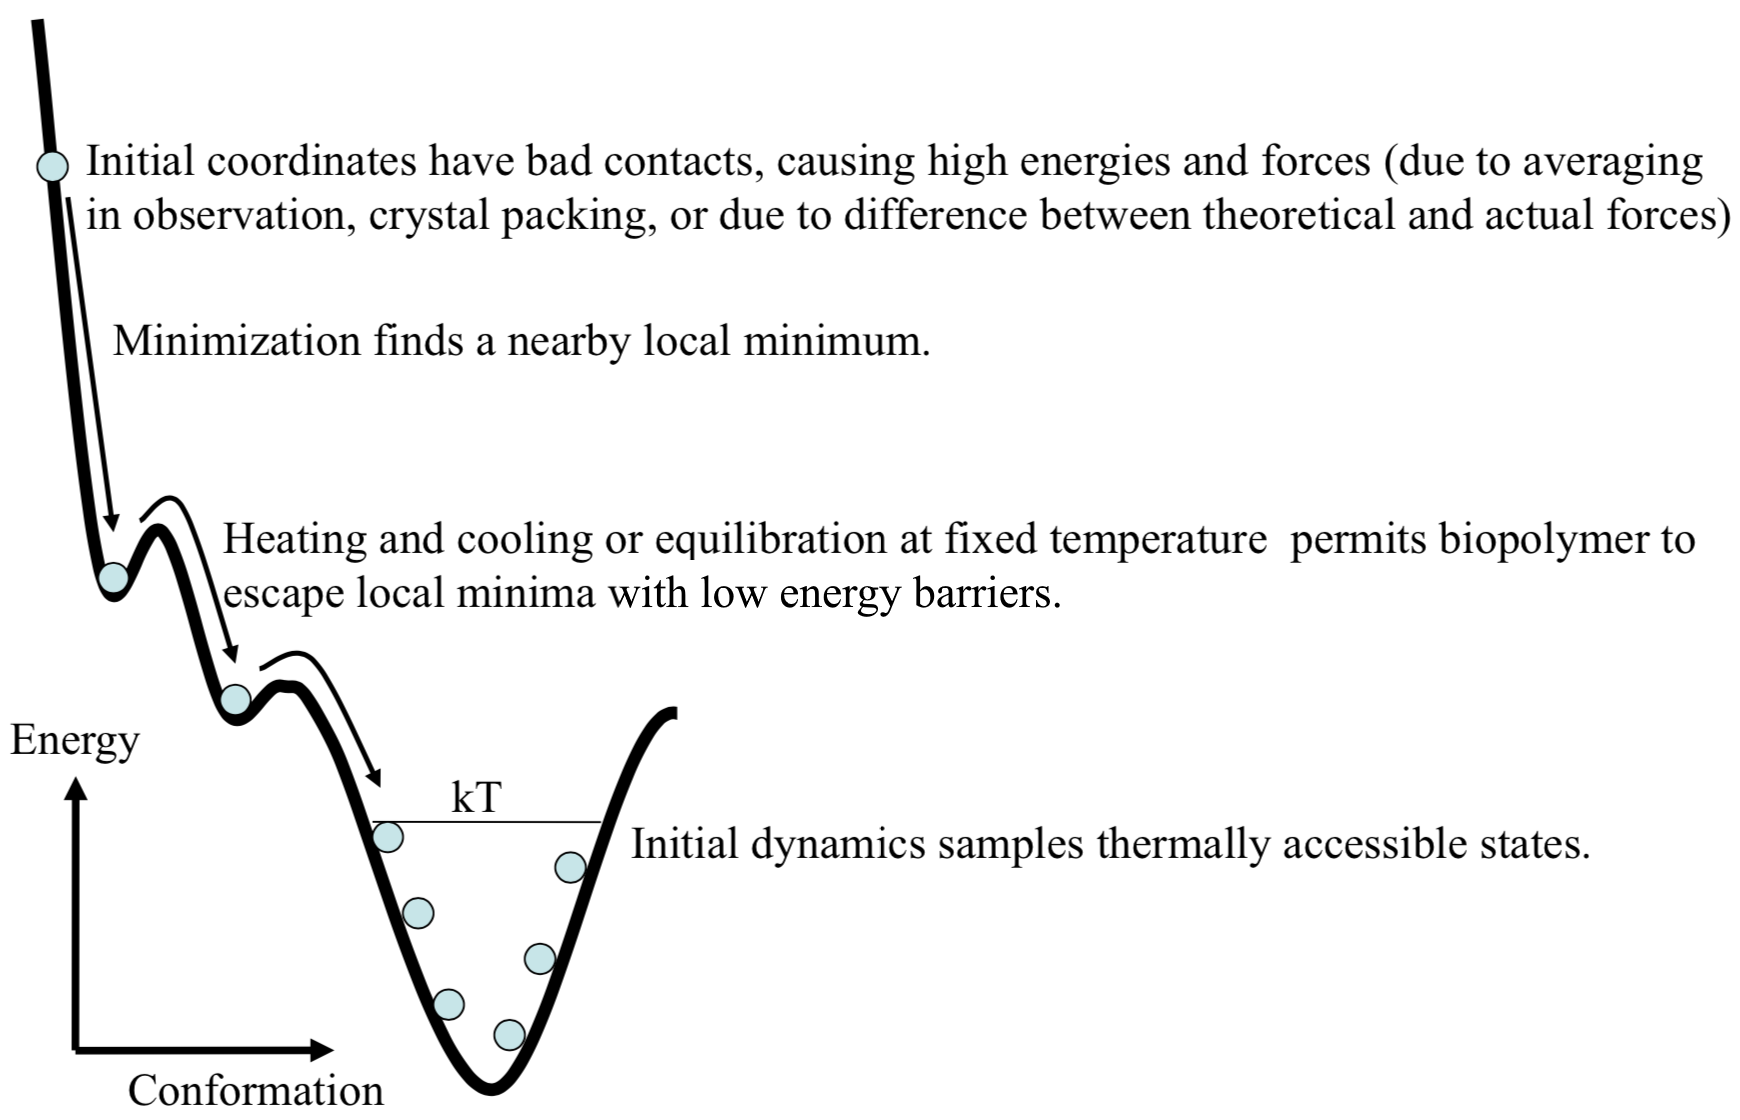
\includegraphics[width=0.9\textwidth]{initial_state-01.png}
    
    \footnotesize{\caption{Schematic representation of the velocity Verlet algorithm. At each steps, the stored variables are in grey boxes.
    \textit{Source:} Allen and Tildesley, \textit{Computer Simulation of Liquids} (1st edition, 1987) 
    \cite{ref:AllenTildesley_1ed}.}
    \label{fig:symplettic-integrator}
    }
\end{minipage} 
\end{figure}



\section{NAMD}
Introduction to NAND envairoment and explanation of its features useful for this study (or, utilezed in this study)

In order to conduct MD simulations, various computer programs have been developed including X-PLOR and CHARMM. These programs were originally developed for serial machines. Simulation of large molecules like protein, however, require enormous computing power. One way to achieve such simulations is to utilize parallel computers. In last 10 years, distributed memory parallel computers have been offering cost-effective computational power. 

NAMD was designed to run efficiently on such parallel machines for simulating large molecules. 

NAMD is a parallel molecular dynamics code for high-performance simulation of large biomolecular systems developed by the Theoretical and Computational Biophysics Group in the Beckman Institute for Advanced Science and Technology at the University of Illinois at Urbana-Champaign. 


NAMD scales to hundreds of processors on high-end parallel platforms, as well as tens of processors on low-cost commodity clusters, and also runs on individual desktop and laptop computers. 

NAMD works with AMBER and CHARMM potential functions, parameters, and file formats. 


On a molecular scale, the fundamental processing units in the living cell are often huge in size and function in an even larger complex environment. Striking progress has been achieved in characterizing the immense machines of the cell, such as the ribosome, at the atomic level. Advances in biomedicine demand tools to model these machines to understand their function and their role in maintaining the health of cells. Accordingly, the purpose of NAMD is to enable high-performance classical simulation of biomolecules in realistic environments of 100,000 atoms or more. The progress made in this regard is illustrated in Figure 1. A decade ago in its first release NAMD permitted simulation of a protein-DNA complex encompassing 36,000 atoms one of the largest simulations carried out at the time. The most recent release permitted the simulation of a protein-DNA complex of 314,000 atoms. To probe the behavior of this 10-fold larger system, the simulated period actually increased 100-fold as well \cite{ref:NAMD}.

\subsection{Introduction - What is NAMD?}

\subsection{Molecular Dynamics Concepts and Algorithms}

\subsection{Configuration File?}

\subsection{Input and Output Files}

\subsection{Force Field Parameters}

\subsection{NAMD's features useful for this study}
%Based on Charm++ parallel objects, NAMD scales to hundreds of cores for typical simulations and beyond 500,000 cores for the largest simulations. NAMD uses the popular molecular graphics program VMD for simulation setup and trajectory analysis, but is also file-compatible with AMBER, CHARMM, and X-PLOR. NAMD is distributed free of charge with source code. You can build NAMD yourself or download binaries for a wide variety of platforms. 







\subsection{Molecular Dynamics Concepts and Algorithms}

\subsection{xxx}


Molecular dynamics (MD) simulations compute atomic trajectories by solving equations of motion numerically using empirical force fields, such as the CHARMM force field, that approximate the actual atomic force in biopolymer systems. Detailed information about MD simulations can be found in several books such as [1, 55]. In order to conduct MD simulations, various computer programs have been developed including X-PLOR [13] and CHARMM [12]. These programs were originally developed for serial machines. Simulation of large molecules, however, require enormous computing power. One way to achieve such simulations is to utilize parallel computers. In recent years, distributed memory parallel computers have been offering cost-effective computational power. NAMD was designed to run efficiently on such parallel machines for simulating large molecules. NAMD is particularly well suited to the increasingly popular Beowulf-class PC clusters, which are quite similar to the workstation clusters for which is was originally designed. Future versions of NAMD will also make efficient use of clusters of multi-processor workstations or PCs.

NAMD has several important features:
\begin{itemize}
\item \textbf{Force Field Compatibility}\\
The force field used by NAMD is the same as that used by the programs CHARMM [12] and X-PLOR [13]. This force field includes local interaction terms consisting of bonded interactions between 2, 3, and 4 atoms and pairwise interactions including electrostatic and van der Waals forces. This commonality allows simulations to migrate between these three programs.
\item \textbf{Efficient Full Electrostatics Algorithms}\\
NAMD incorporates the Particle Mesh Ewald (PME) algorithm, which takes the full electrostatic interactions into account. This algorithm reduces the computational complexity of electrostatic force evaluation from O($N^2$) to O($N \, \text{log} \, N$).
\item \textbf{Multiple Time Stepping}\\
The velocity Verlet integration method is used to advance the positions and velocities of the atoms in time. To further reduce the cost of the evaluation of long-range electrostatic forces, a multiple time step scheme is employed. The local interactions (bonded, van der Waals and electrostatic interactions within a specified distance) are calculated at each time step. The longer range interactions (electrostatic interactions beyond the specified distance) are only computed less often. This amortizes the cost of computing the electrostatic forces over several timesteps. A smooth splitting function is used to separate a quickly varying short-range portion of the electrostatic interaction from a more slowly varying long-range component. It is also possible to employ an intermediate timestep for the short-range non- bonded interactions, performing only bonded interactions every timestep.
\item \textbf{Input and Output Compatibility}\\
The input and output file formats used by NAMD are identical to those used by CHARMM and X-PLOR. Input formats include coordinate files in PDB format [6], structure files in X-PLOR PSF format, and energy parameter files in either CHARMM or X-PLOR formats. Output formats include PDB coordinate files and binary DCD trajectory files. These similarities assure that the molecular dynamics trajectories from NAMD can be read by CHARMM or X-PLOR and that the user can exploit the many analysis algorithms of the latter packages.
\item \textbf{Dynamics Simulation Options}\\
MD simulations may be carried out using several options, including:
\begin{itemize}
\item[$\circ$] Constant energy dynamics,
\item[$\circ$] Constant temperature dynamics via: velocity rescaling, velocity reassignment or Langevin dynamics.
\item[$\circ$] Periodic boundary conditions,
\item[$\circ$] Constant pressure dynamics via: Berendsen pressure coupling or Nos\'{e}-Hoover Langevin piston
\item[$\circ$] Energy minimization,
\item[$\circ$] Fixed atoms,
\item[$\circ$] Rigid waters,
\item[$\circ$] Rigid bonds to hydrogen,
\item[$\circ$] Harmonic restraints,
\item[$\circ$] Spherical or cylindrical boundary restraints.
\end{itemize}
\item \textbf{Easy to Modify and Extend}\\
Another primary design objective for NAMD is extensibility and maintainability. In order to achieve this, it is designed in an object-oriented style with C++. Since molecular dynamics is a new field, new algorithms and techniques are continually being developed. NAMD’s modular design allows one to integrate and test new algorithms easily. If you are contemplating a particular modification to NAMD you are encouraged to contact the developers for guidance.
\item \textbf{Interactive MD simulations}\\
A system undergoing simulation in NAMD may be viewed and altered with VMD; for instance, forces can be applied to a set of atoms to alter or rearrange part of the molecular structure. For more information on VMD, see \url{http://www.ks.uiuc.edu/Research/vmd/}.
\item \textbf{Load Balancing}\\
An important factor in parallel applications is the equal distribution of computational load among the processors. In parallel molecular simulation, a spatial decomposition that evenly distributes the computational load causes the region of space mapped to each processor to become very irregular, hard to compute and difficult to generalize to the evaluation of many different types of forces. NAMD addresses this problem by using a simple uniform spatial decomposition where the entire model is split into uniform cubes of space called patches. An initial load balancer assigns patches and the calculation of interactions among the atoms within them to processors such that the computational load is balanced as much as possible. During the simulation, an incremental load balancer monitors the load and performs necessary adjustments.
\end{itemize}

\section{VMD}
VMD (Visual Molecular Dynamics) is a molecular visualization and analysis program designed for biological systems such as proteins, nucleic acids, lipid bilayer assemblies, etc. The program is developed by the Theoretical and Computational Biophysics Group at the University of Illinois at Urbana-Champaign. Among molecular graphics programs, VMD is unique in its ability to efficiently operate on large biomolecular complexes and long-timescale molecular dynamics trajectories, its interoperability with a large number of molecular dynamics simulation tools, its integration of structure and sequence information, and its built-in support for advanced image rendering and movie making.

Key features of VMD include:
\begin{itemize}
\item General 3-D molecular visualization with extensive drawing and coloring methods and strong support for visualization of molecular dynamics
\item Supports all major molecular data file formats, with no limits to structure or trajectory sizes except memory capacity and addressing
\item Extensive atom selection syntax for choosing subsets of atoms for both analytical tasks and for graphical display
\item Visualization of volumetric data
\item Molecular analysis commands
\item Rendering of high-resolution, publication-quality molecule images
\item Built-in movie making tools
\item Building and preparing systems for molecular dynamics simulations
\item Interactive molecular dynamics simulations
\item User-extensible through the built-in Tcl and Python scripting languages
\item Extensible source code written in C and C++
\end{itemize}
